\appendix

\chapter{PLC Program}  \label{app:plcProg}
    This appendix contains a printout of the \acrshort{plc} program. The first two pages are the Main Program and the proceeding are the subroutines. All subroutines are called from the Main Program.

    \begin{description}
        \item[Main Program:] Pages 1 - 2
        \item[Sort:] Pages 3 - 6
        \item[Dispense:] Page 7
        \item[Alarm:] Pages 8 - 13
        \item[Modbus:] Page 14
        \item[Arduino:] Page 15
        \item[Inputs:] Pages 16- 18
        \item[Outputs:] Pages 19 - 21
        \item[System:] Pages 22- 23
    \end{description}

    NOTE: Page numbers are associated with the \acrshort{plc} printout numbers shown in the bottom right corner. 
    
    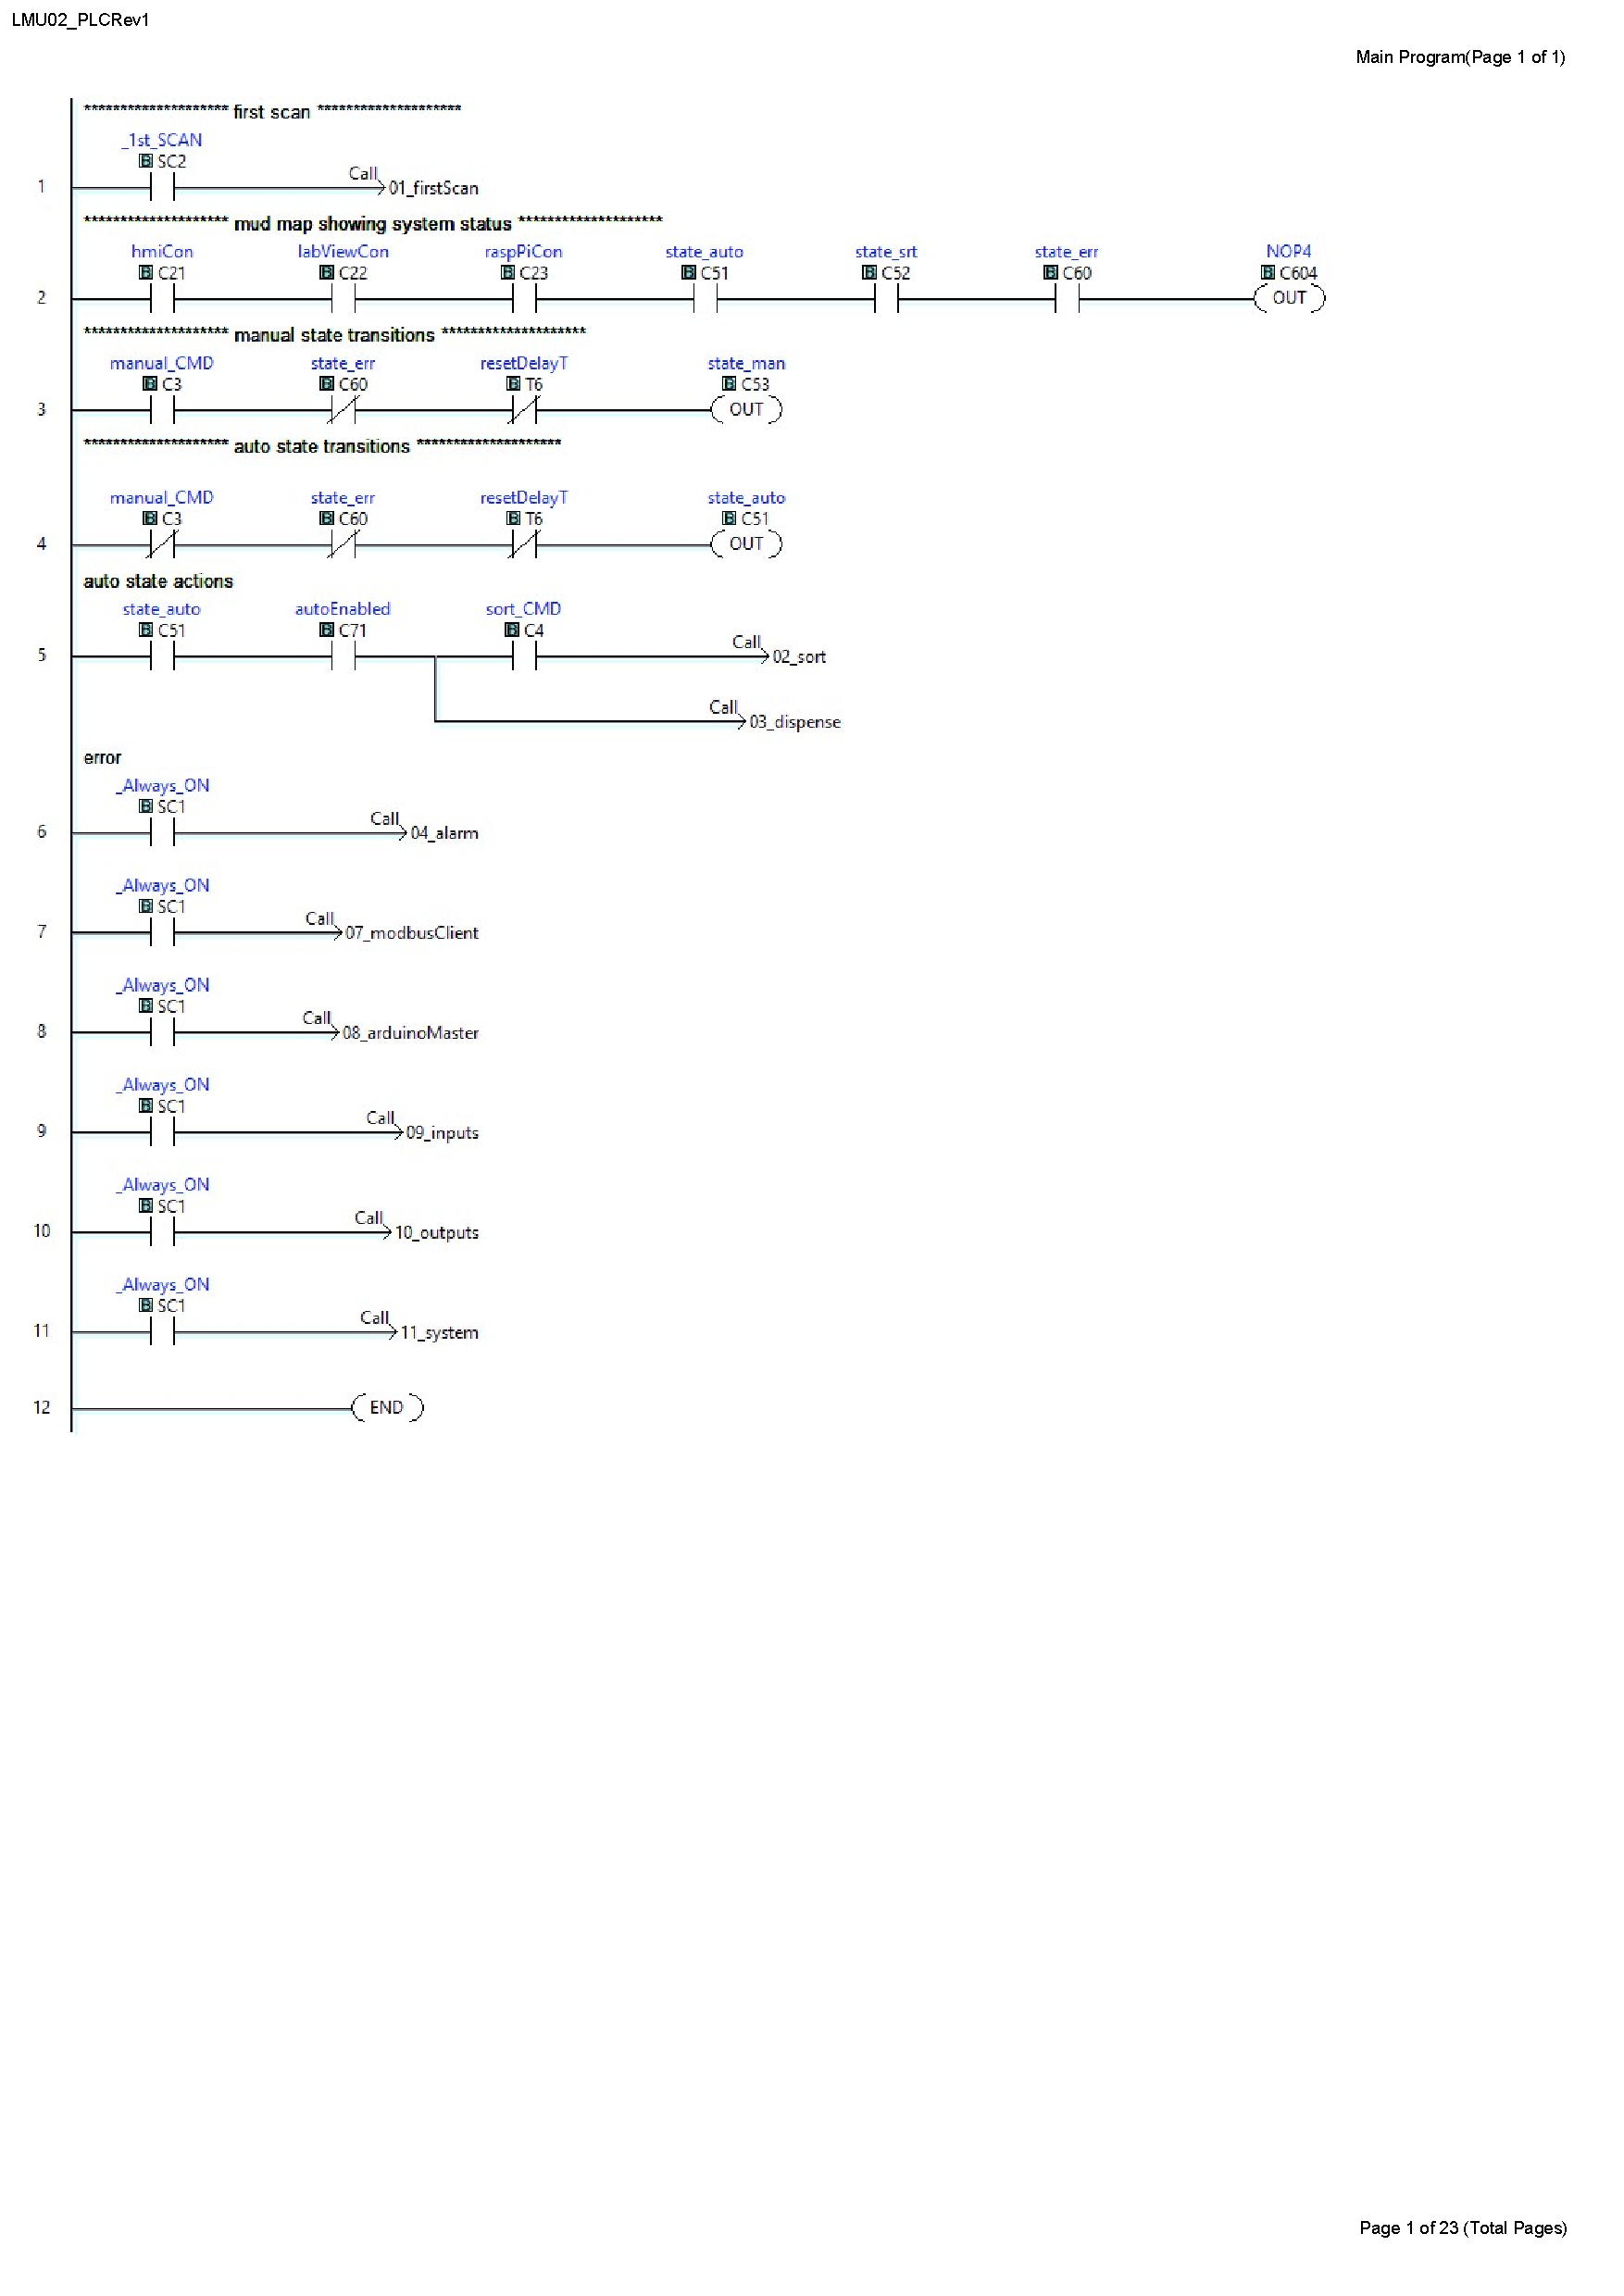
\includepdf[pages=-]{3_appendix/PLC_Program.pdf} 
    
\chapter{Electrical Schematics} \label{app:elecSch}
    This appendix provides the electrical schematics of the lolly machine. \acrshort{io} tags match what is in the \acrshort{plc} to allow for easy cross referencing. These drawings have been made with TinyCad.
    \begin{figure}[H]
    \centering
    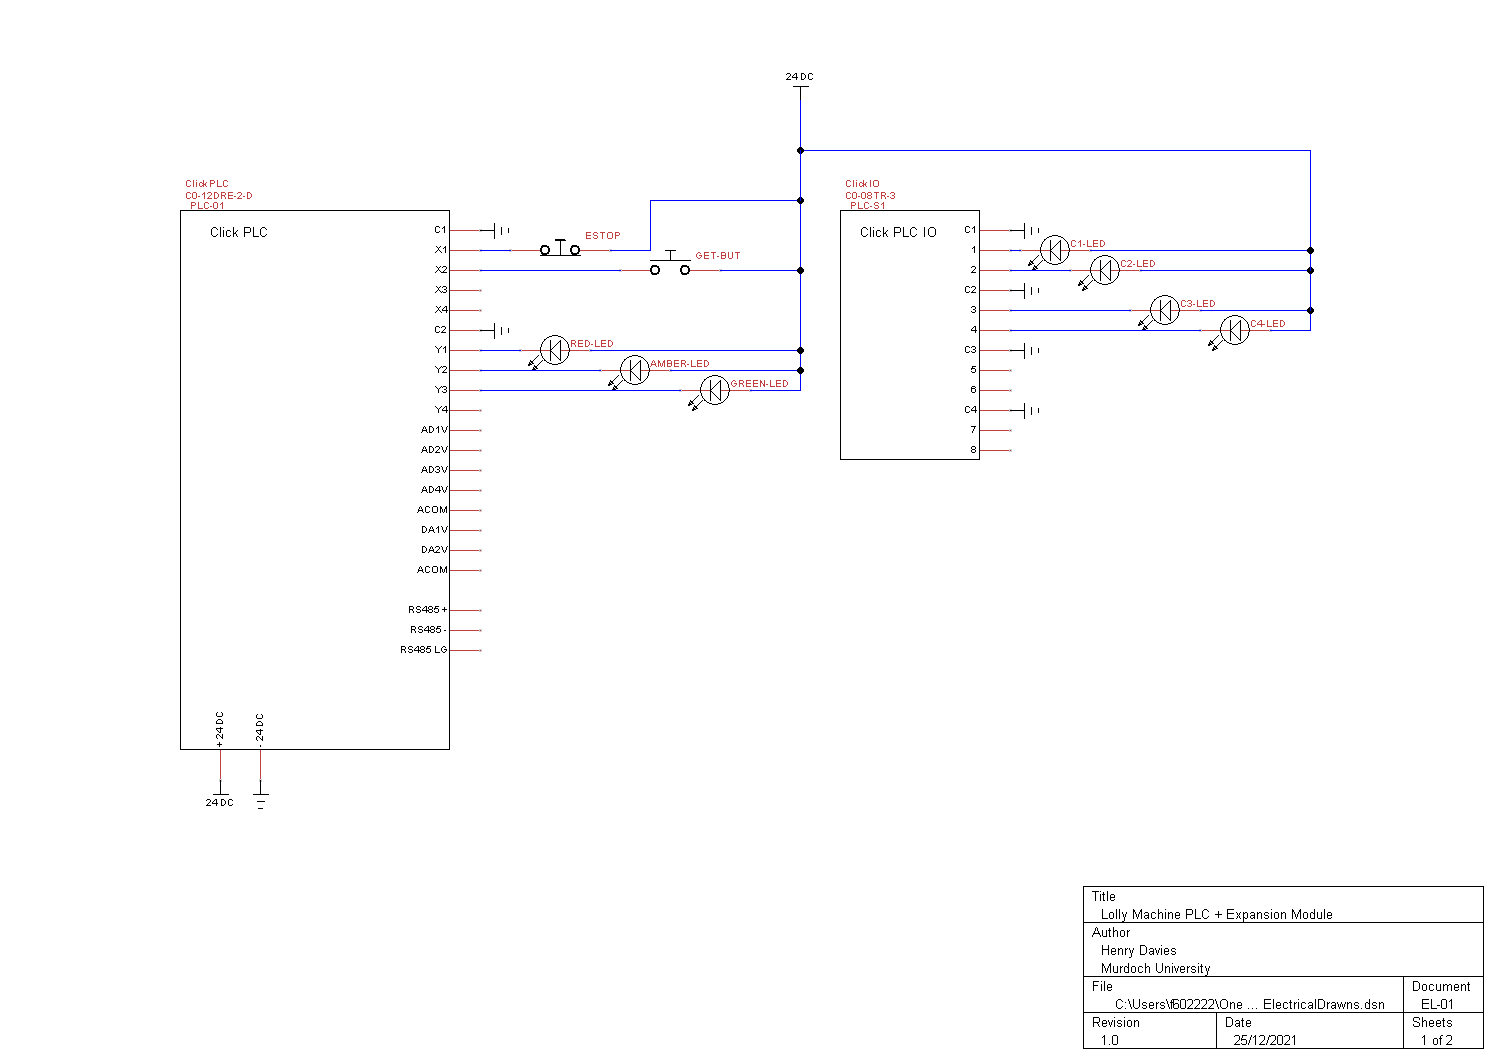
\includegraphics[width = 1\textwidth]{2_images/ElectricalDrawns01}
    \caption{Electrical schematic showing the PLC and I/O.}
    \label{fig:ElectricalDrawns01}
\end{figure} 

\begin{figure}[H]
    \centering
    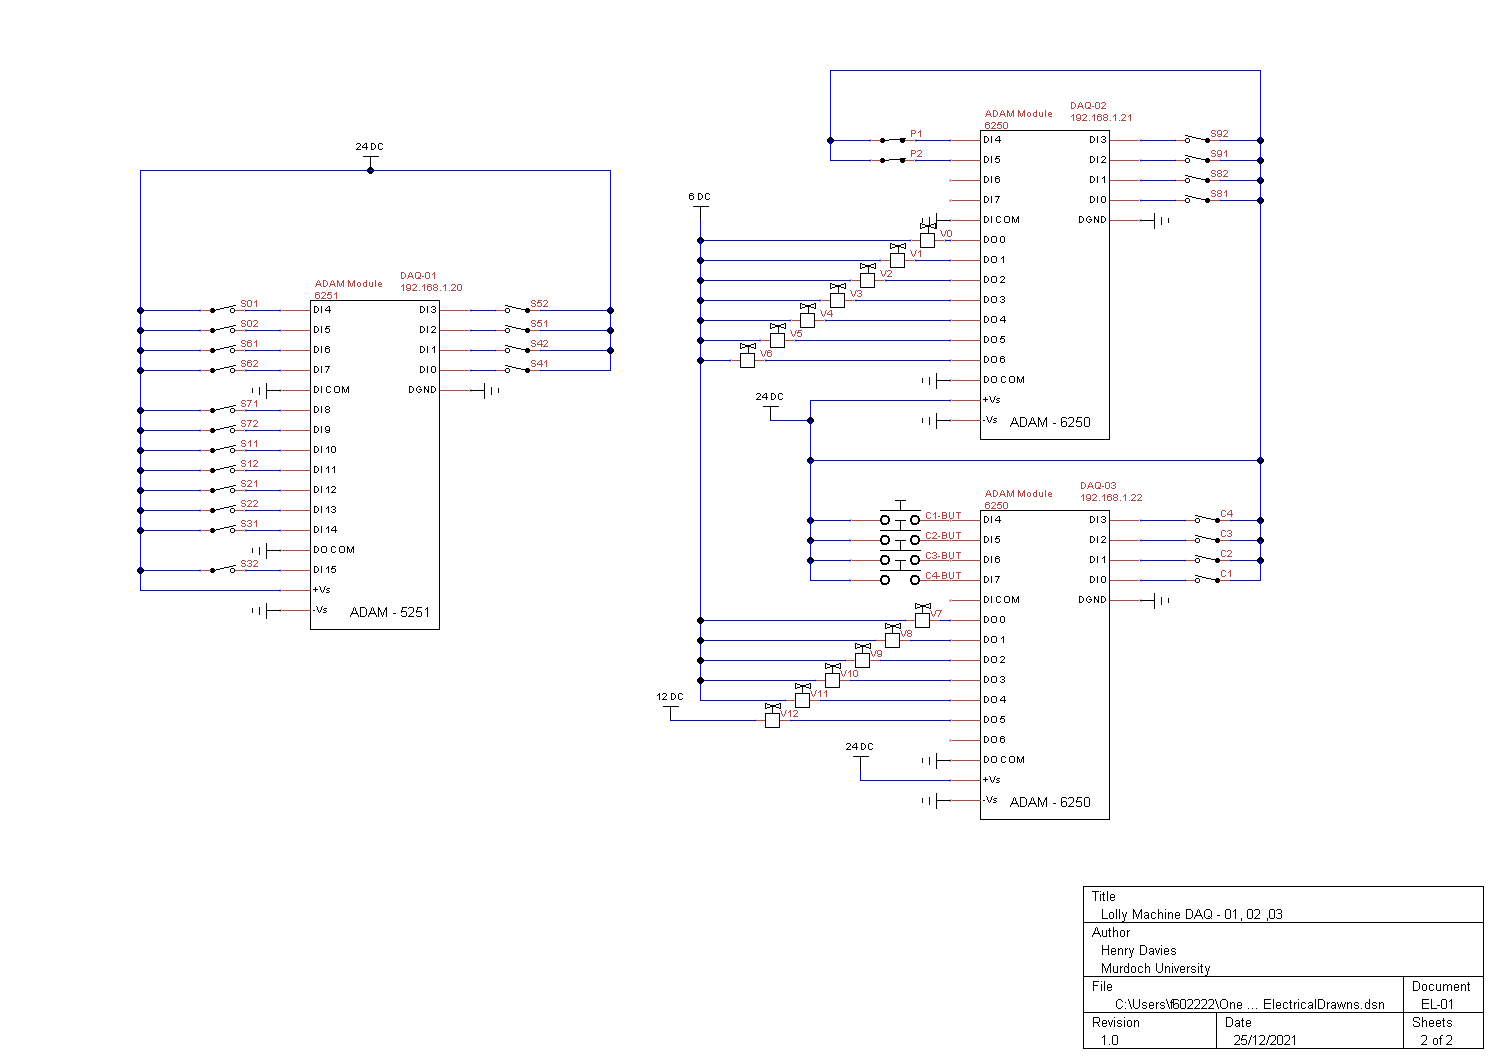
\includegraphics[width = 1\textwidth]{2_images/ElectricalDrawns02}
    \caption{Electrical schematic showing DAQ modules and I/O.}
    \label{fig:ElectricalDrawns02}
\end{figure} 

\chapter{User Manual} \label{app:userGuide}
    This appendix is the user manual. It contains instructions on how to use the machine from each control source along with some basic machine information.
    

\begin{figure}[ht]
    \centering
    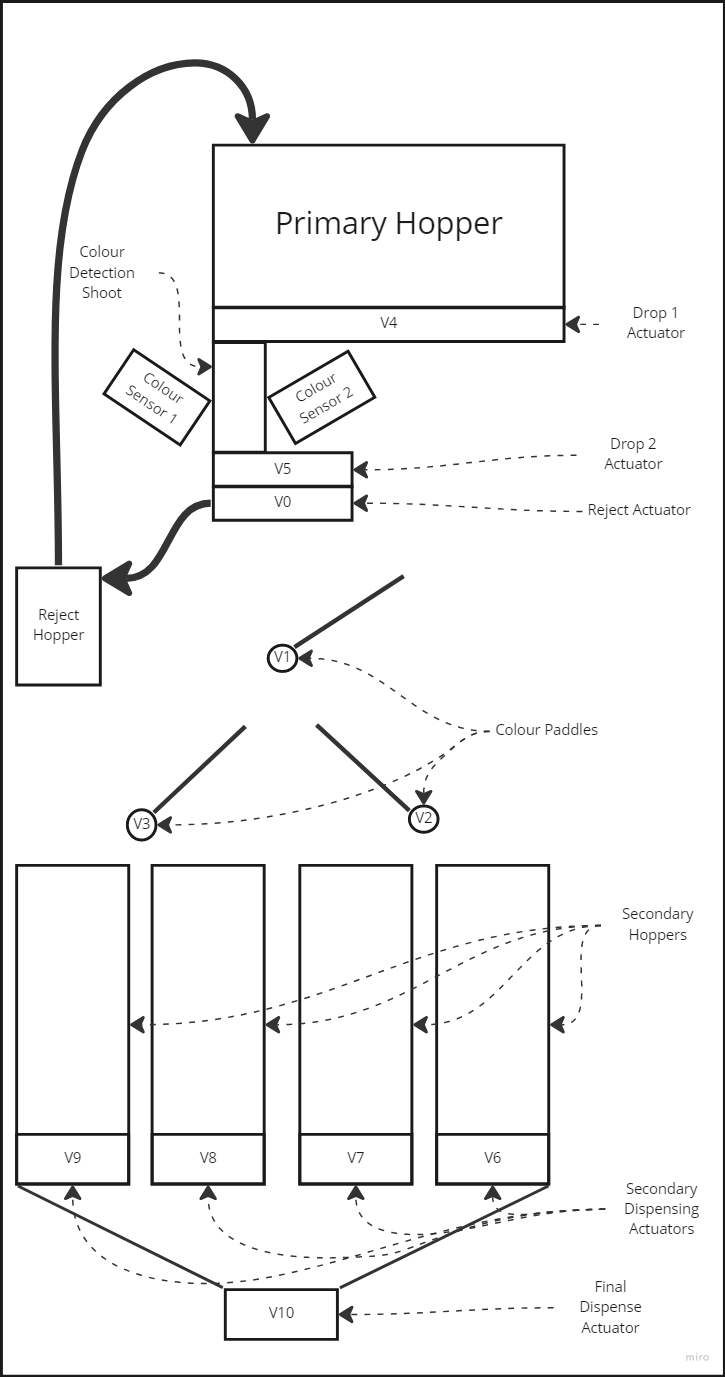
\includegraphics[scale = 0.3]{2_images/lollyMachineBw}
    \caption{General arrangement of the lolly machine.}
    \label{fig:lollyMachineBw}
\end{figure}

\section{Introduction}

    Welcome to the lolly machine user guide. This guide contains basic instructions on how to use the lolly machine. This guide is split into four different sections - one containing general machine information and one for each control source. 


\section{Lolly Machine - General Information}

    \subsection{Start Up}
        \begin{enumerate}
            \item Connect the machine to a pneumatic air supply. Preferably shop-air. 
            \item Plug the machine into a  10 amp general purpose outlet(power point).
            \item Turn on the pneumatic supply valve then open the pressure regulator on the lolly machine so that it reads approximately 90 psig.
            \item Switch on the general purpose outlet.
        \end{enumerate}
        
        The lolly machine is now ready for operation. \newline
        NOTE: When the lolly machine first starts up it is common to get multiple FTO and FTC faults. These are easily cleared and acknowledged via the either of the HMIs.
        
 

    \subsection{Operating Modes}
        The lolly machine has three different modes of operation which are outlined in the descriptions below.

            \subsubsection{ALARM MODE} While in the alarm mode, the machine is inoperable. This is to prevent any unwanted/ unexpected movement. The machine will go into alarm mode when an alarm is activated. There are two three types of alarms on the lolly machine.
            \begin{enumerate}
                \item\textbf{FTO:} Fail to Open. An FTO alarm will occur in the event that a valve fails to open.
                \item\textbf{FTC:} Fail to Close. An FTC alarm will occur in the event that a valve fails to close.
                \item\textbf{E-STOP:} Then machine will alarm if the emergency stop button is pressed.
            \end{enumerate}
            
           \subsubsection{MANUAL MODE}
                While in manual mode, valves on the lolly machine are manually driven. None of the automatic functions work while in manual. 
                
            \subsubsection{AUTOMATIC MODE}
                If the machine is enabled in automatic mode, the sort and dispense functions are available. Enabling the machine in automatic mode is achievable through each of the HMIs.
                \begin{description}
                    \item[Sort] The machine will sort lollies as a function of colour from the primary hopper to the secondary hoppers.
                    \item[Dispense] The machine will dispense lollies from the secondary hoppers to the user.
                \end{description}
                
    \subsection{Traffic Light Indicator Key}          
        \begin{description}
            \item[Red Solid] Alarm Mode. When in this state the machine will not run. 
            \item[Amber Solid] Manual Mode.
            \item[Green Flashing]  Automatic Mode - Not Enabled
            \item[Green Solid]  Automatic Mode - Enabled
        \end{description}

    
    
\section{Siemens HMI}
    The Siemens HMI is physically mounted to the front panel and is intended to be the main HMI of the machine. Various machine functions can be achieved through this HMI.
    
    \subsection{F Keys}
        \begin{description}
        \item[F1:] Go to home screen
            \item[F2:] Go to play screen
            \item[F3:] Spare 
            \item[F4:] Spare
            \item[F5:] Toggle sorting program
            \item[F6:] Reset/ acknowledge alarms
            
            The `F' keys have been intentionally left unlabeled to discourage younger users from pressing the buttons. 
        \end{description}  
    

    \subsection{Alarm}
        When an alarm is active, an alarm popup will appear on the screen showing the alarm details. To clear the alarms, press the F1 button. The alarms must then be acknowledged by pressing the `\!' button.
    \subsection{Manual Operation}
        To operate the machine in manual mode follow the proceeding steps: 
            \begin{enumerate}
                \item Go to the home screen by pressing F1.
                \item Ensure that the HMI is the connected control source (Text of the `Control Source' window is highlighted green)
                \item Press the `Mode' button so the `Manual' indicator underneath is green. 
                \item Press the `Manual' button located in the `Screens' window - this will open the `Manual' screen.
                \item Press the valve buttons to toggle them on and off. The buttons will be change colour depending on the state of the valve.
            \end{enumerate}

    \subsection{Automatic Operation}
        To use the machine in automatic mode, follow the proceeding steps. 
            \begin{enumerate}
                \item Go to the home screen by pressing F1.
                \item Ensure that the HMI is the connected control source (Text of the `Control Source' window is highlighted green)
                \item Press the `Mode' button so the `Auto.' indicator underneath is green.
                \item Enable the machine by pressing the `ON' button in the `Auto. Control' window.
                \item Press the F2 button any time while the machine is enabled in automatic mode to toggle the sorting program. 
                \item Press F2 or the `Play' button in the `Screens' window to open the play time screen.
                \item Select the desired lollies by pressing the lolly colour buttons (four buttons in the middle of the page with a coloured circle housed in a grey box). Once the lolly colours have been selected, press the `GET IT' button to dispense said lollies. Only one of each colour lolly can be dispensed at a time. 
                \item To disable the automatic functions, press the `OFF' button in the `Auto.Control' window. If it's an emergency, press the emergency stop button on the side of the machine. 
            \end{enumerate}
        \subsection{IO Status}
            The IO status of the machine can be viewed at anytime regardless as to the operating mode and control source. The IO status page is read only and is accessible on the Siemens HMI through the proceeding steps. 

        \begin{enumerate}
            \item Go to the home screen by pressing F1.
            \item Press the `IO' button located within the Screens `window'.
        \end{enumerate}
            
            
\section{LabVIEW Application}
        A LabVIEW application to control and monitor the lolly machine has also been developed. This interface has been built with an intuitive design to allow operators to easily troubleshoot and diagnose problems.
        
    \subsection{Setup} 
        \begin{enumerate}
            \item Set the static IP address of the EWS to 192.168.113.
            \item Open the LabVIEW run-time program.
            \item Run the LabVIEW run-time program.
        \end{enumerate}
        
    \subsection{General Operation}
        Once the LabVIEW application has been opened a text window with multiple tabs provides instruction on how to use the application. 
        
\section{Node-RED Dashboard}
    A Node-RED service running on a Raspberry Pi provides a method of control, accessible via WiFi enabled devices.
    Once connected to the Node-RED dashboard, there are two main tabs - one for control and one to view I/O status. 
    
    \subsection{Setup}
        \begin{enumerate}
            \item Connect to the Raspberry Pi WiFi
            \begin{description}
                \item Network Name: Lolly Machine
                \item Password: iwantcandy
            \end{description}
            \item Open a web browser (preferably Chrome, Safari, Edge or Mozilla Firefox)
            \item Go to \href{https://192.168.1.120:1880/ui}{192.168.1.120:1880/ui}
            \item Welcome to the Node-RED dashboard for the lolly machine. 
        \end{enumerate}
        
    \subsection{Alarm}
        If the `ALARM' indicator underneath the General header is red, an alarm is active. First try to reset the alarm by pressing the `RESET button under the `General' header. If this doesn't work, check the HMI mounted to the front of the lolly machine for a detailed description of the alarm.
    
    \subsection{Manual Operation}
            To operate the machine in manual mode, follow the proceeding steps. 
            \begin{enumerate}
                \item Go to the `Control' tab.
                \item Ensure that `Node-RED' is selected under the `Control Source' header. If it is not selected, press `REQUEST CONTROL' under the `General' header. 
                \item Move the `Auto/ Manual' slider under the `General' header to the right.
                \item To toggle outputs, move the desired sliders under the `Manual' header.
            \end{enumerate}

        \subsection{Automatic Operation}
            To operate the machine in automatic mode, follow the proceeding steps. 
            \begin{enumerate}
                \item Go to the `Control' tab
                \item Ensure that `Node-RED' is selected under the `Control Source' header. If it is not selected, press `REQUEST CONTROL' under the `General' header. 
                \item Move the `Auto/ Manual' slider under the `General' header to the left.
                \item To enable the machine in automatic mode, press the `ON' button under the `Auto.' header. 
                \item Move the `Sort' slider under the `Auto.' header at any time while automatic mode is enabled to toggle the sorting program.
                \item Select the desired lollies by pressing the `COL.[1-4]' buttons under the `Auto' header. Once the lolly colours have been selected, press the ‘GET’ button to dispense said lollies. Only one of each colour lolly can be dispensed at a time.
                \item To disable automatic functions, press the `OFF' button under the `Auto.' header. If it's an emergency, press the emergency stop button on the side of the machine.
            \end{enumerate}

            \subsection{IO Status}
                To view the I/O status, open the `IO Status' tab. This tab is organised into four different columns with the following headers. 
                \begin{description}
                    \item Proximity Sensors
                    \item Valves
                    \item Colour Sensors
                    \item Auto Switches
                \end{description}

        





\chapter{IO List} \label{app:ioList}
    This \acrshort{io} list provides information about all physical \acrshort{io} onboard the lolly machine. Please note, the Address refers to the \acrshort{plc} address.
    \begin{center}
    \begin{longtable}[c]{ |c|c|c|c|c|c| }
        \caption{I/O list}\\
        \hline
        \textbf{IO}	&	\textbf{Adddress}	&	\textbf{Type}	&	\textbf{Desc.}	&	\textbf{Location} & \textbf{Connected Device}\\
        S41	&	C201	&	Input - WET	&	Auto Switch	&	Candy Drop	&	DAQ-01:DI 00\\
        S42	&	C202	&	Input - WET	&	Auto Switch	&	Candy Drop	&	DAQ-01:DI 01\\
        S51	&	C203	&	Input - WET	&	Auto Switch	&	Accept Candy	&	DAQ-01:DI 0\\
        S52	&	C204	&	Input - WET	&	Auto Switch	&	Accept Candy	&	DAQ-01:DI 0\\
        S01	&	C205	&	Input - WET	&	Auto Switch	&	Reject Candy	&	DAQ-01:DI 0\\
        S02	&	C206	&	Input - WET	&	Auto Switch	&	Reject Candy	&	DAQ-01:DI 0\\
        S61	&	C207	&	Input - WET	&	Auto Switch	&	Colour 1	&	DAQ-01:DI 06\\
        S62	&	C208	&	Input - WET	&	Auto Switch	&	Colour 1	&	DAQ-01:DI 07\\
        S71	&	C209	&	Input - WET	&	Auto Switch	&	Colour 2	&	DAQ-01:DI 08\\
        S72	&	C210	&	Input - WET	&	Auto Switch	&	Colour 2	&	DAQ-01:DI 09\\
        S11	&	C211	&	Input - WET	&	Auto Switch	&	Top Paddle	&	DAQ-01:DI 10\\
        S12	&	C212	&	Input - WET	&	Auto Switch	&	Top Paddle	&	DAQ-01:DI 11\\
        S21	&	C213	&	Input - WET	&	Auto Switch	&	Right Paddle	&	DAQ-01:DI 1\\
        S22	&	C214	&	Input - WET	&	Auto Switch	&	Right Paddle	&	DAQ-01:DI 1\\
        S31	&	C215	&	Input - WET	&	Auto Switch	&	Left Paddle	&	DAQ-01:DI 14\\
        S32	&	C216	&	Input - WET	&	Auto Switch	&	Left Paddle	&	DAQ-01:DI 15\\
        S81	&	C217	&	Input - WET	&	Auto Switch	&	Colour 3	&	DAQ-02:DI 0\\
        S82	&	C218	&	Input - WET	&	Auto Switch	&	Colour 3	&	DAQ-02:DI 1\\
        S91	&	C219	&	Input - WET	&	Auto Switch	&	Colour 4	&	DAQ-02:DI 2\\
        S92	&	C220	&	Input - WET	&	Auto Switch	&	Colour 4	&	DAQ-02:DI 3\\
        P1	&	C221	&	Input - WET	&	Prox. Sens.	&	Colour Shoot	&	DAQ-02:DI 4\\
        P2	&	C222	&	Input - WET	&	Prox. Sens.	&	Reject Bucket	&	DAQ-02:DI 5\\
        V0	&	C225	&	Output - SINK	&	Valve - Rot.	&	Reject Candy	&	DAQ-02: DO 0\\
        V1	&	C226	&	Output - SINK	&	Valve - Rot.	&	Top Paddle	&	DAQ-02: DO 1\\
        V2	&	C227	&	Output - SINK	&	Valve - Rot.	&	Right Paddle	&	DAQ-02: DO 2\\
        V3	&	C228	&	Output - SINK	&	Valve - Rot.	&	Left Paddle	&	DAQ-02: DO 3\\
        V4	&	C229	&	Output - SINK	&	Valve - Lin.	&	Candy Drop	&	DAQ-02: DO 4\\
        V5	&	C230	&	Output - SINK	&	Valve Lin.	&	Accept Candy	&	DAQ-02: DO 5\\
        V6	&	C231	&	Output - SINK	&	Valve - Rot.	&	Colour 4	&	DAQ-02: DO 6\\
        C1	&	C232	&	Input - WET	&	Colour 1	&	Colour Sensor CS1	&	DAQ-03: DI 0\\
        C2	&	C233	&	Input - WET	&	Colour 2	&	Colour Sensor CS3	&	DAQ-03: DI 1\\
        C3	&	C234	&	Input - WET	&	Colour 3	&	Colour Sensor CS3	&	DAQ-03: DI 2\\
        C4	&	C235	&	Input - WET	&	Colour 4	&	Colour Sensor CS3	&	DAQ-03: DI 3\\
        C1-BUT	&	C236	&	Input - WET	&	C1 Button	&	Front Panel	&	DAQ-03: DI 4\\
        C2-BUT	&	C237	&	Input - WET	&	C2 Button	&	Front Panel	&	DAQ-03: DI 5\\
        C3-BUT	&	C238	&	Input - WET	&	C3 Button	&	Front Panel	&	DAQ-03: DI 6\\
        C4-BUT	&	C239	&	Input - WET	&	C45 Button	&	Front Panel	&	DAQ-03: DI 7\\
        V7	&	C240	&	Output - SINK	&	Valve - Rot.	&	Colour Paddle 3	&	DAQ-03 DO 0\\
        V8	&	C241	&	Output - SINK	&	Valve - Rot.	&	Colour Paddle 2	&	DAQ-03 DO 1\\
        V9	&	C242	&	Output - SINK	&	Valve - Rot.	&	Colour Paddle 1	&	DAQ-03 DO 2\\
        V10	&	C243	&	Output - SINK	&	Valve - Lin.	&	Dispense Candy	&	DAQ-03 DO 3\\
        V11	&	C244	&	Output - SINK	&	Pneumatic Line	&	Reject Shoot	&	DAQ-03 DO 4\\
        V12	&	C245	&	Output - SINK	&	Shoot Unblocker	&	Colour Detection Shoot	& DAQ-03 DO 5\\
        ESTOP	&	X1	&	Input - WET	&	E Stop Button	&	Side Panel	&	PLC-01:X1\\
        GET-BUT	&	X2	&	Input - WET	&	Get Button	&	Front Panel	&	PLC-01:X2\\
        RED-LED	&	Y1	&	Output - SINK	&	Red LED	&	Mid Panel	&	PLC-01:Y1\\
        AMBER-LED	&	Y2	&	Output - SINK	&	Amber LED	&	Mid Panel	&	PLC-01:Y2\\
        GREEN-LED	&	Y3	&	Output - SINK	&	Green LED	&	Mid Panel	&	PLC-01:Y3\\
        C1-LED	&	Y101	&	Output - SINK	&	Colour 1 LED	&	Front Panel	&	PLC-S1:1\\
        C2-LED	&	Y102	&	Output - SINK	&	Colour 2 LED	&	Front Panel	&	PLC:S1:2\\
        C3-LED	&	Y103	&	Output - SINK	&	Colour 3 LED	&	Front Panel	&	PLC:S1:3\\
        C4-LED	&	Y104	&	Output - SINK	&	Colour 4 LED	&	Front Panel	&	PLC:S1:4\\
        GET-LED	&	Y105	&	Output - SINK	&	GET LED	&	Front Panel	&	PLC-S1:5\\
        \hline
    \end{longtable}
\end{center}
\label{table:ioList}

\chapter{Modbus Register} \label{app:modbusRegister}
    This appendix contains the Modbus and associated \acrshort{plc} addresses for all program variables. This list can be used as a reference for future development.
    

\begin{center}
    \begin{longtable}[c]{ |c|c|c|c|c| }
        \caption{Modbus register and PLC address list}\\
        \hline
        \textbf{PLC Address}	&	\textbf{Data Type}	&	\textbf{Modbus Address}	&	\textbf{Function Code}	&	\textbf{Nickname}\\ 
        \hline
        X001	&	BIT	&	100001	&	FC=02	&	eStop\\
        X002	&	BIT	&	100002	&	FC=02	&	getBut\\
        Y001	&	BIT	&	8193	&	FC=01,05,15	&	redLed\\
        Y002	&	BIT	&	8194	&	FC=01,05,15	&	amberLed\\
        Y003	&	BIT	&	8195	&	FC=01,05,15	&	greenLed\\
        Y101	&	BIT	&	8225	&	FC=01,05,15	&	col1Led\\
        Y102	&	BIT	&	8226	&	FC=01,05,15	&	col2Led\\
        Y103	&	BIT	&	8227	&	FC=01,05,15	&	col3Led\\
        Y104	&	BIT	&	8228	&	FC=01,05,15	&	col4Led\\
        Y105	&	BIT	&	8229	&	FC=01,05,15	&	getLed\\
        C1	&	BIT	&	16385	&	FC=01,05,15	&	autoEnable\_CMD\\
        C2	&	BIT	&	16386	&	FC=01,05,15	&	autoDisable\_CMD\\
        C3	&	BIT	&	16387	&	FC=01,05,15	&	manual\_CMD\\
        C4	&	BIT	&	16388	&	FC=01,05,15	&	sort\_CMD\\
        C5	&	BIT	&	16389	&	FC=01,05,15	&	C5\_CMD\\
        C6	&	BIT	&	16390	&	FC=01,05,15	&	C6\_CMD\\
        C7	&	BIT	&	16391	&	FC=01,05,15	&	C7\_CMD\\
        C8	&	BIT	&	16392	&	FC=01,05,15	&	C8\_CMD\\
        C9	&	BIT	&	16393	&	FC=01,05,15	&	C9\_CMD\\
        C10	&	BIT	&	16394	&	FC=01,05,15	&	reset\_CMD\\
        C11	&	BIT	&	16395	&	FC=01,05,15	&	C11\_CMD\\
        C12	&	BIT	&	16396	&	FC=01,05,15	&	col1\_CMD\\
        C13	&	BIT	&	16397	&	FC=01,05,15	&	col2\_CMD\\
        C14	&	BIT	&	16398	&	FC=01,05,15	&	col3\_CMD\\
        C15	&	BIT	&	16399	&	FC=01,05,15	&	col4\_CMD\\
        C16	&	BIT	&	16400	&	FC=01,05,15	&	get\_CMD\\
        C21	&	BIT	&	16405	&	FC=01,05,15	&	hmiCon\\
        C22	&	BIT	&	16406	&	FC=01,05,15	&	labViewCon\\
        C23	&	BIT	&	16407	&	FC=01,05,15	&	raspPiCon\\
        C24	&	BIT	&	16408	&	FC=01,05,15	&	hmiDiscon\\
        C25	&	BIT	&	16409	&	FC=01,05,15	&	labViewDiscon\\
        C26	&	BIT	&	16410	&	FC=01,05,15	&	nodRedDiscon\\
        C31	&	BIT	&	16415	&	FC=01,05,15	&	auto\_V0\\
        C32	&	BIT	&	16416	&	FC=01,05,15	&	auto\_V1\\
        C33	&	BIT	&	16417	&	FC=01,05,15	&	auto\_V2\\
        C34	&	BIT	&	16418	&	FC=01,05,15	&	auto\_V3\\
        C35	&	BIT	&	16419	&	FC=01,05,15	&	auto\_V4\\
        C36	&	BIT	&	16420	&	FC=01,05,15	&	auto\_V5\\
        C37	&	BIT	&	16421	&	FC=01,05,15	&	auto\_V6\\
        C38	&	BIT	&	16422	&	FC=01,05,15	&	auto\_V7\\
        C39	&	BIT	&	16423	&	FC=01,05,15	&	auto\_V8\\
        C40	&	BIT	&	16424	&	FC=01,05,15	&	auto\_V9\\
        C41	&	BIT	&	16425	&	FC=01,05,15	&	auto\_V10\\
        C42	&	BIT	&	16426	&	FC=01,05,15	&	auto\_V11\\
        C43	&	BIT	&	16427	&	FC=01,05,15	&	auto\_V12\\
        C51	&	BIT	&	16435	&	FC=01,05,15	&	state\_auto\\
        C52	&	BIT	&	16436	&	FC=01,05,15	&	state\_srt\\
        C53	&	BIT	&	16437	&	FC=01,05,15	&	state\_man\\
        C60	&	BIT	&	16444	&	FC=01,05,15	&	state\_err\\
        C71	&	BIT	&	16455	&	FC=01,05,15	&	autoEnabled\\
        C81	&	BIT	&	16465	&	FC=01,05,15	&	err\_V0\_fto\\
        C82	&	BIT	&	16466	&	FC=01,05,15	&	err\_V0\_ftc\\
        C83	&	BIT	&	16467	&	FC=01,05,15	&	err\_V1\_fto\\
        C84	&	BIT	&	16468	&	FC=01,05,15	&	err\_V1\_ftc\\
        C85	&	BIT	&	16469	&	FC=01,05,15	&	err\_V2\_fto\\
        C86	&	BIT	&	16470	&	FC=01,05,15	&	err\_V2\_ftc\\
        C87	&	BIT	&	16471	&	FC=01,05,15	&	err\_V3\_fto\\
        C88	&	BIT	&	16472	&	FC=01,05,15	&	err\_V3\_ftc\\
        C89	&	BIT	&	16473	&	FC=01,05,15	&	err\_V4\_fto\\
        C90	&	BIT	&	16474	&	FC=01,05,15	&	err\_V4\_ftc\\
        C91	&	BIT	&	16475	&	FC=01,05,15	&	err\_V5\_fto\\
        C92	&	BIT	&	16476	&	FC=01,05,15	&	err\_V5\_ftc\\
        C93	&	BIT	&	16477	&	FC=01,05,15	&	err\_V6\_fto\\
        C94	&	BIT	&	16478	&	FC=01,05,15	&	err\_V6\_ftc\\
        C95	&	BIT	&	16479	&	FC=01,05,15	&	err\_V7\_fto\\
        C96	&	BIT	&	16480	&	FC=01,05,15	&	err\_V7\_ftc\\
        C97	&	BIT	&	16481	&	FC=01,05,15	&	err\_V8\_fto\\
        C98	&	BIT	&	16482	&	FC=01,05,15	&	err\_V8\_ftc\\
        C99	&	BIT	&	16483	&	FC=01,05,15	&	err\_V9\_fto\\
        C100	&	BIT	&	16484	&	FC=01,05,15	&	err\_V9\_ftc\\
        C101	&	BIT	&	16485	&	FC=01,05,15	&	clientConnection Error\\
        C121	&	BIT	&	16505	&	FC=01,05,15	&	sort\_drop1\\
        C122	&	BIT	&	16506	&	FC=01,05,15	&	sort\_checkColour\\
        C123	&	BIT	&	16507	&	FC=01,05,15	&	sort\_colour1\\
        C124	&	BIT	&	16508	&	FC=01,05,15	&	sort\_colour2\\
        C125	&	BIT	&	16509	&	FC=01,05,15	&	sort\_colour3\\
        C126	&	BIT	&	16510	&	FC=01,05,15	&	sort\_colour4\\
        C127	&	BIT	&	16511	&	FC=01,05,15	&	sort\_colourBad\\
        C128	&	BIT	&	16512	&	FC=01,05,15	&	sort\_drop2\\
        C129	&	BIT	&	16513	&	FC=01,05,15	&	sort\_noLolly\\
        C130	&	BIT	&	16514	&	FC=01,05,15	&	sort\_entryBit\\
        C131	&	BIT	&	16515	&	FC=01,05,15	&	sort\_droppedShoot\\
        C171	&	BIT	&	16555	&	FC=01,05,15	&	disp\_memBit1\\
        C172	&	BIT	&	16556	&	FC=01,05,15	&	disp\_memBit2\\
        C201	&	BIT	&	16585	&	FC=01,05,15	&	S41\\
        C202	&	BIT	&	16586	&	FC=01,05,15	&	S42\\
        C203	&	BIT	&	16587	&	FC=01,05,15	&	S51\\
        C204	&	BIT	&	16588	&	FC=01,05,15	&	S52\\
        C205	&	BIT	&	16589	&	FC=01,05,15	&	S01\\
        C206	&	BIT	&	16590	&	FC=01,05,15	&	S02\\
        C207	&	BIT	&	16591	&	FC=01,05,15	&	S61\\
        C208	&	BIT	&	16592	&	FC=01,05,15	&	S62\\
        C209	&	BIT	&	16593	&	FC=01,05,15	&	S71\\
        C210	&	BIT	&	16594	&	FC=01,05,15	&	S72\\
        C211	&	BIT	&	16595	&	FC=01,05,15	&	S11\\
        C212	&	BIT	&	16596	&	FC=01,05,15	&	S12\\
        C213	&	BIT	&	16597	&	FC=01,05,15	&	S21\\
        C214	&	BIT	&	16598	&	FC=01,05,15	&	S22\\
        C215	&	BIT	&	16599	&	FC=01,05,15	&	S31\\
        C216	&	BIT	&	16600	&	FC=01,05,15	&	S32\\
        C217	&	BIT	&	16601	&	FC=01,05,15	&	S81\\
        C218	&	BIT	&	16602	&	FC=01,05,15	&	S82\\
        C219	&	BIT	&	16603	&	FC=01,05,15	&	S91\\
        C220	&	BIT	&	16604	&	FC=01,05,15	&	S92\\
        C221	&	BIT	&	16605	&	FC=01,05,15	&	P1\\
        C222	&	BIT	&	16606	&	FC=01,05,15	&	P2\\
        C223	&	BIT	&	16607	&	FC=01,05,15	&	DAQ02\_DI 6\\
        C224	&	BIT	&	16608	&	FC=01,05,15	&	DAQ02\_DI 7\\
        C225	&	BIT	&	16609	&	FC=01,05,15	&	V0\\
        C226	&	BIT	&	16610	&	FC=01,05,15	&	V1\\
        C227	&	BIT	&	16611	&	FC=01,05,15	&	V2\\
        C228	&	BIT	&	16612	&	FC=01,05,15	&	V3\\
        C229	&	BIT	&	16613	&	FC=01,05,15	&	V4\\
        C230	&	BIT	&	16614	&	FC=01,05,15	&	V5\\
        C231	&	BIT	&	16615	&	FC=01,05,15	&	V6\\
        C232	&	BIT	&	16616	&	FC=01,05,15	&	C1\\
        C233	&	BIT	&	16617	&	FC=01,05,15	&	C2\\
        C234	&	BIT	&	16618	&	FC=01,05,15	&	C3\\
        C235	&	BIT	&	16619	&	FC=01,05,15	&	C4\\
        C236	&	BIT	&	16620	&	FC=01,05,15	&	C1But\\
        C237	&	BIT	&	16621	&	FC=01,05,15	&	C2But\\
        C238	&	BIT	&	16622	&	FC=01,05,15	&	C3But\\
        C239	&	BIT	&	16623	&	FC=01,05,15	&	C4But\\
        C240	&	BIT	&	16624	&	FC=01,05,15	&	V7\\
        C241	&	BIT	&	16625	&	FC=01,05,15	&	V8\\
        C242	&	BIT	&	16626	&	FC=01,05,15	&	V9\\
        C243	&	BIT	&	16627	&	FC=01,05,15	&	V10\\
        C244	&	BIT	&	16628	&	FC=01,05,15	&	V11\\
        C245	&	BIT	&	16629	&	FC=01,05,15	&	V12\\
        C246	&	BIT	&	16630	&	FC=01,05,15	&	DAQ03\_DO 6\\
        C301	&	BIT	&	16685	&	FC=01,05,15	&	modHmi\_b1\\
        C302	&	BIT	&	16686	&	FC=01,05,15	&	modHmi\_b2\\
        C303	&	BIT	&	16687	&	FC=01,05,15	&	modHmi\_b3\\
        C304	&	BIT	&	16688	&	FC=01,05,15	&	modHmi\_b4\\
        C305	&	BIT	&	16689	&	FC=01,05,15	&	modHmi\_b5\\
        C306	&	BIT	&	16690	&	FC=01,05,15	&	modHmi\_b6\\
        C307	&	BIT	&	16691	&	FC=01,05,15	&	modHmi\_b7\\
        C308	&	BIT	&	16692	&	FC=01,05,15	&	modHmi\_b8\\
        C309	&	BIT	&	16693	&	FC=01,05,15	&	modHmi\_b9\\
        C310	&	BIT	&	16694	&	FC=01,05,15	&	modHmi\_b10\\
        C311	&	BIT	&	16695	&	FC=01,05,15	&	modHmi\_b11\\
        C312	&	BIT	&	16696	&	FC=01,05,15	&	modHmi\_b12\\
        C313	&	BIT	&	16697	&	FC=01,05,15	&	modHmi\_b13\\
        C314	&	BIT	&	16698	&	FC=01,05,15	&	modHmi\_b14\\
        C315	&	BIT	&	16699	&	FC=01,05,15	&	modHmi\_b15\\
        C316	&	BIT	&	16700	&	FC=01,05,15	&	modHmi\_b16\\
        C321	&	BIT	&	16705	&	FC=01,05,15	&	modHmi\_V0\\
        C322	&	BIT	&	16706	&	FC=01,05,15	&	modHmi\_V1\\
        C323	&	BIT	&	16707	&	FC=01,05,15	&	modHmi\_V2\\
        C324	&	BIT	&	16708	&	FC=01,05,15	&	modHmi\_V3\\
        C325	&	BIT	&	16709	&	FC=01,05,15	&	modHmi\_V4\\
        C326	&	BIT	&	16710	&	FC=01,05,15	&	modHmi\_V5\\
        C327	&	BIT	&	16711	&	FC=01,05,15	&	modHmi\_V6\\
        C328	&	BIT	&	16712	&	FC=01,05,15	&	modHmi\_V7\\
        C329	&	BIT	&	16713	&	FC=01,05,15	&	modHmi\_V8\\
        C330	&	BIT	&	16714	&	FC=01,05,15	&	modHmi\_V9\\
        C331	&	BIT	&	16715	&	FC=01,05,15	&	modHmi\_V10\\
        C332	&	BIT	&	16716	&	FC=01,05,15	&	modHmi\_V11\\
        C333	&	BIT	&	16717	&	FC=01,05,15	&	modHmi\_V12\\
        C341	&	BIT	&	16725	&	FC=01,05,15	&	modLab\_b1\\
        C342	&	BIT	&	16726	&	FC=01,05,15	&	modLab\_b2\\
        C343	&	BIT	&	16727	&	FC=01,05,15	&	modLab\_b3\\
        C344	&	BIT	&	16728	&	FC=01,05,15	&	modLab\_b4\\
        C345	&	BIT	&	16729	&	FC=01,05,15	&	modLab\_b5\\
        C346	&	BIT	&	16730	&	FC=01,05,15	&	modLab\_b6\\
        C347	&	BIT	&	16731	&	FC=01,05,15	&	modLab\_b7\\
        C348	&	BIT	&	16732	&	FC=01,05,15	&	modLab\_b8\\
        C349	&	BIT	&	16733	&	FC=01,05,15	&	modLab\_b9\\
        C350	&	BIT	&	16734	&	FC=01,05,15	&	modLab\_b10\\
        C351	&	BIT	&	16735	&	FC=01,05,15	&	modLab\_b11\\
        C352	&	BIT	&	16736	&	FC=01,05,15	&	modLab\_b12\\
        C353	&	BIT	&	16737	&	FC=01,05,15	&	modLab\_b13\\
        C354	&	BIT	&	16738	&	FC=01,05,15	&	modLab\_b14\\
        C355	&	BIT	&	16739	&	FC=01,05,15	&	modLab\_b15\\
        C356	&	BIT	&	16740	&	FC=01,05,15	&	modLab\_b16\\
        C361	&	BIT	&	16745	&	FC=01,05,15	&	modLab\_V0\\
        C362	&	BIT	&	16746	&	FC=01,05,15	&	modLab\_V1\\
        C363	&	BIT	&	16747	&	FC=01,05,15	&	modLab\_V2\\
        C364	&	BIT	&	16748	&	FC=01,05,15	&	modLab\_V3\\
        C365	&	BIT	&	16749	&	FC=01,05,15	&	modLab\_V4\\
        C366	&	BIT	&	16750	&	FC=01,05,15	&	modLab\_V5\\
        C367	&	BIT	&	16751	&	FC=01,05,15	&	modLab\_V6\\
        C368	&	BIT	&	16752	&	FC=01,05,15	&	modLab\_V7\\
        C369	&	BIT	&	16753	&	FC=01,05,15	&	modLab\_V8\\
        C370	&	BIT	&	16754	&	FC=01,05,15	&	modLab\_V9\\
        C371	&	BIT	&	16755	&	FC=01,05,15	&	modLab\_V10\\
        C372	&	BIT	&	16756	&	FC=01,05,15	&	modLab\_V11\\
        C373	&	BIT	&	16757	&	FC=01,05,15	&	modLab\_V12\\
        C381	&	BIT	&	16765	&	FC=01,05,15	&	modRasp\_b1\\
        C382	&	BIT	&	16766	&	FC=01,05,15	&	modRasp\_b2\\
        C383	&	BIT	&	16767	&	FC=01,05,15	&	modRasp\_b3\\
        C384	&	BIT	&	16768	&	FC=01,05,15	&	modRasp\_b4\\
        C385	&	BIT	&	16769	&	FC=01,05,15	&	modRasp\_b5\\
        C386	&	BIT	&	16770	&	FC=01,05,15	&	modRasp\_b6\\
        C387	&	BIT	&	16771	&	FC=01,05,15	&	modRasp\_b7\\
        C388	&	BIT	&	16772	&	FC=01,05,15	&	modRasp\_b8\\
        C389	&	BIT	&	16773	&	FC=01,05,15	&	modRasp\_b9\\
        C390	&	BIT	&	16774	&	FC=01,05,15	&	modRasp\_b10\\
        C391	&	BIT	&	16775	&	FC=01,05,15	&	modRasp\_b11\\
        C392	&	BIT	&	16776	&	FC=01,05,15	&	modRasp\_b12\\
        C393	&	BIT	&	16777	&	FC=01,05,15	&	modRasp\_b13\\
        C394	&	BIT	&	16778	&	FC=01,05,15	&	modRasp\_b14\\
        C395	&	BIT	&	16779	&	FC=01,05,15	&	modRasp\_b15\\
        C396	&	BIT	&	16780	&	FC=01,05,15	&	modRasp\_b16\\
        C401	&	BIT	&	16785	&	FC=01,05,15	&	modRasp\_V0\\
        C402	&	BIT	&	16786	&	FC=01,05,15	&	modRasp\_V1\\
        C403	&	BIT	&	16787	&	FC=01,05,15	&	modRasp\_V2\\
        C404	&	BIT	&	16788	&	FC=01,05,15	&	modRasp\_V3\\
        C405	&	BIT	&	16789	&	FC=01,05,15	&	modRasp\_V4\\
        C406	&	BIT	&	16790	&	FC=01,05,15	&	modRasp\_V5\\
        C407	&	BIT	&	16791	&	FC=01,05,15	&	modRasp\_V6\\
        C408	&	BIT	&	16792	&	FC=01,05,15	&	modRasp\_V7\\
        C409	&	BIT	&	16793	&	FC=01,05,15	&	modRasp\_V8\\
        C410	&	BIT	&	16794	&	FC=01,05,15	&	modRasp\_V9\\
        C411	&	BIT	&	16795	&	FC=01,05,15	&	modRasp\_V10\\
        C412	&	BIT	&	16796	&	FC=01,05,15	&	modRasp\_V11\\
        C413	&	BIT	&	16797	&	FC=01,05,15	&	modRasp\_V12\\
        C501	&	BIT	&	16885	&	FC=01,05,15	&	modDaq1\_recv\\
        C502	&	BIT	&	16886	&	FC=01,05,15	&	modDaq1\_recvSucc\\
        C503	&	BIT	&	16887	&	FC=01,05,15	&	modDaq1\_recvErr\\
        C504	&	BIT	&	16888	&	FC=01,05,15	&	modDaq2\_recv\\
        C505	&	BIT	&	16889	&	FC=01,05,15	&	modDaq2\_recvSucc\\
        C506	&	BIT	&	16890	&	FC=01,05,15	&	modDaq2\_recvErr\\
        C507	&	BIT	&	16891	&	FC=01,05,15	&	modDaq2\_send\\
        C508	&	BIT	&	16892	&	FC=01,05,15	&	modDaq2\_sendSucc\\
        C509	&	BIT	&	16893	&	FC=01,05,15	&	modDaq2\_sendErr\\
        C510	&	BIT	&	16894	&	FC=01,05,15	&	modDaq3\_recv\\
        C511	&	BIT	&	16895	&	FC=01,05,15	&	modDaq3\_recvSucc\\
        C512	&	BIT	&	16896	&	FC=01,05,15	&	modDaq3\_recvErr\\
        C513	&	BIT	&	16897	&	FC=01,05,15	&	modDaq3\_send\\
        C514	&	BIT	&	16898	&	FC=01,05,15	&	modDaq3\_sendSucc\\
        C515	&	BIT	&	16899	&	FC=01,05,15	&	modDaq3\_sendErr\\
        C530	&	BIT	&	16914	&	FC=01,05,15	&	rs485\_1Send\\
        C531	&	BIT	&	16915	&	FC=01,05,15	&	rs485\_1Succ\\
        C532	&	BIT	&	16916	&	FC=01,05,15	&	rs485\_2Send\\
        C533	&	BIT	&	16917	&	FC=01,05,15	&	rs485\_2Succ\\
        C534	&	BIT	&	16918	&	FC=01,05,15	&	rs485\_3Send\\
        C535	&	BIT	&	16919	&	FC=01,05,15	&	rs485\_3Succ\\
        C536	&	BIT	&	16920	&	FC=01,05,15	&	rs485\_4Send\\
        C537	&	BIT	&	16921	&	FC=01,05,15	&	rs485\_4Succ\\
        C601	&	BIT	&	16985	&	FC=01,05,15	&	NOP1\\
        C602	&	BIT	&	16986	&	FC=01,05,15	&	NOP2\\
        C603	&	BIT	&	16987	&	FC=01,05,15	&	NOP3\\
        C604	&	BIT	&	16988	&	FC=01,05,15	&	NOP4\\
        T1	&	BIT	&	145057	&	FC=02	&	dispDelTimer\\
        T2	&	BIT	&	145058	&	FC=02	&	hmi\_watchDogTimer1\\
        T3	&	BIT	&	145059	&	FC=02	&	hmi\_watchDogTimer2\\
        T4	&	BIT	&	145060	&	FC=02	&	2SecTimer\_1\\
        T5	&	BIT	&	145061	&	FC=02	&	2SecTimer\_2\\
        T6	&	BIT	&	145062	&	FC=02	&	resetDelayT\\
        T61	&	BIT	&	145117	&	FC=02	&	V0\_fto\\
        T62	&	BIT	&	145118	&	FC=02	&	V0\_ftc\\
        T63	&	BIT	&	145119	&	FC=02	&	V1\_fto\\
        T64	&	BIT	&	145120	&	FC=02	&	V1\_ftc\\
        T65	&	BIT	&	145121	&	FC=02	&	V2\_fto\\
        T66	&	BIT	&	145122	&	FC=02	&	V2\_ftc\\
        T67	&	BIT	&	145123	&	FC=02	&	V3\_fto\\
        T68	&	BIT	&	145124	&	FC=02	&	V3\_ftc\\
        T69	&	BIT	&	145125	&	FC=02	&	V4\_fto\\
        T70	&	BIT	&	145126	&	FC=02	&	V4\_ftc\\
        T71	&	BIT	&	145127	&	FC=02	&	V5\_fto\\
        T72	&	BIT	&	145128	&	FC=02	&	V5\_ftc\\
        T73	&	BIT	&	145129	&	FC=02	&	V6\_fto\\
        T74	&	BIT	&	145130	&	FC=02	&	V6\_ftc\\
        T75	&	BIT	&	145131	&	FC=02	&	V7\_fto\\
        T76	&	BIT	&	145132	&	FC=02	&	V7\_ftc\\
        T77	&	BIT	&	145133	&	FC=02	&	V8\_fto\\
        T78	&	BIT	&	145134	&	FC=02	&	V8\_ftc\\
        T79	&	BIT	&	145135	&	FC=02	&	V9\_fto\\
        T80	&	BIT	&	145136	&	FC=02	&	V9\_ftc\\
        T121	&	BIT	&	145177	&	FC=02	&	sort\_newLollyTON\\
        T122	&	BIT	&	145178	&	FC=02	&	sort\_blockedShootTON1\\
        T123	&	BIT	&	145179	&	FC=02	&	sort\_blockedShootTON2\\
        CT20	&	BIT	&	149172	&	FC=02	&	modbus\_CT\\
        CT21	&	BIT	&	149173	&	FC=02	&	rs485\_CT\\
        SC1	&	BIT	&	161441	&	FC=02	&	\_Always\_ON\\
        SC2	&	BIT	&	161442	&	FC=02	&	\_1st\_SCAN\\
        SC5	&	BIT	&	161445	&	FC=02	&	\_100ms\_Clock\\
        SC6	&	BIT	&	161446	&	FC=02	&	\_500ms\_Clock\\
        SC7	&	BIT	&	161447	&	FC=02	&	\_1sec\_Clock\\
        DS1	&	INT	&	400001	&	FC=03,06,16	&	alarmCode1\\
        DS2	&	INT	&	400002	&	FC=03,06,16	&	alarmCode2\\
        DS5	&	INT	&	400005	&	FC=03,06,16	&	hmi\_heartBeat\\
        DS7	&	INT	&	400007	&	FC=03,06,16	&	labView\_watchdog\\
        DS8	&	INT	&	400008	&	FC=03,06,16	&	labView\_watchDogMem\\
        DS9	&	INT	&	400009	&	FC=03,06,16	&	nodeRed\_watchDog\\
        DS10	&	INT	&	400010	&	FC=03,06,16	&	nodeRed\_watchDogMem\\
        CTD20	&	INT2	&	449191	&	FC=03,06,16	&	modClinetSeq\\
        CTD21	&	INT2	&	449193	&	FC=03,06,16	&	rs485Seq\\
        SD50	&	INT	&	461490	&	FC=03,06,16	&	\_Port2\_Received\_Data\_L\\
        SD60	&	INT	&	461500	&	FC=03,06,16	&	\_Port3\_Received\_Data\_L\\
        \hline
    \end{longtable}
\end{center}
\label{table:modbusRegister}

\chapter{HMI Alarm List} \label{app:alarmList}
    This is the alarm list for the Siemens KTP600 \acrshort{hmi}. This table has been generated by exporting the Alarm list through \acrshort{tia} Portal. 
    

\begin{table}[H]
\caption{Siemens Alarm List}
\begin{center}
    \begin{tabular}{ |c|c|c|c|c|c| }
        \hline
        \textbf{ID}	& \textbf{Name}	& \textbf{Alarm text} &	\textbf{Class} & \textbf{Trigger tag} & \textbf{Trigger bit}\\ 
        \hline
        1 & V0\_fto & V0 fail to open &	Errors & alarmCode1	& 0\\
        2 &	V0\_ftc & V0 fail to close &	Errors & alarmCode1	& 1\\
        3 &	V1\_fto & V1 fail to open & Errors &	alarmCode1	& 2\\
        4 &	V1\_ftc & V1 fail to close &	Errors & alarmCode1	& 3\\
        5 &	V2\_fto & V2 fail to open &	Errors & alarmCode1	& 4\\
        6 &	V2\_ftc & V2 fail to close &	Errors & alarmCode1	& 5\\
        7 &	V3\_fto & V3 fail to open &	Errors & alarmCode1	& 6\\
        8 &	V3\_ftc & V3 fail to close &	Errors & alarmCode1	& 7\\
        9 &	V4\_fto & V4 fail to open &	Errors & alarmCode1	& 8\\
        10 & V4\_ftc & V4 fail to close & Errors	& alarmCode1 & 9\\
        11 & V5\_fto & V5 fail to open &	Errors & alarmCode1	& 10\\
        12 & V5\_ftc & V5 fail to close & Errors	& alarmCode1 & 11\\
        13 & V6\_fto & V6 fail to open &	Errors & alarmCode1	& 12\\
        14 & V6\_ftc & V6 fail to close & Errors & alarmCode1 & 13\\
        15 & V7\_fto & V7 fail to open &	Errors & alarmCode1	& 14\\
        16 & V7\_ftc & V7 fail to close & Errors	& alarmCode1 & 15\\
        17 & V8\_fto & V8 fail to open &	Errors & alarmCode2	& 0\\
        18 & V8\_ftc & V8 fail to close & Errors	& alarmCode2 & 1\\
        19 & V9\_fto & V9 fail to open &	Errors & alarmCode2	& 2\\
        20 & V9\_ftc & V9 fail to close & Errors	& alarmCode2 & 3\\
        22 & E\_STOP & Emergency stop button pressed	& Errors & alarmCode2 & 4\\
        \hline
    \end{tabular}\\
\end{center}
\label{table:alarmList}
\end{table}



\chapter{Arduino Code} \label{app:arduino}
    This appendix contains two separate scripts. The first (Listing \ref{list:arduinoCode1}) is what is currently on the Arduino and controls the RGB strip lights from a RS-485 signal from the PLC. The second (\ref{list:arduinoCode2}) randomly changes the colour of each RGB within the strip at rate of 2 Hz. 
    

\begin{lstlisting}[language=C, caption = Lolly machine arduino code., label=list:arduinoCode1]
#include "FastLED.h"
    // number of LEDs in the strip
    #define NUM_LEDS 60
    // define the data pin on the Arduino
    #define DATA_PIN 3
    // define the clock pin on the Arduino
    #define CLOCK_PIN 13
    // define variables
    long data;
    int bytesAtPort;
    byte r,g,b;
    int lollyCol = 1;
    int i;
    // create led object
    CRGB leds[NUM_LEDS];
    void setup() { 
          FastLED.addLeds<P9813, DATA_PIN, CLOCK_PIN, RGB>(leds, NUM_LEDS);
          Serial.begin(9600);
          Serial.setTimeout(500);
    }
    void loop() { 
    
      if (Serial.available() > 0) {
    	  
    	// check to see how many bytes are at port - diagnostics  
        bytesAtPort = Serial.available();
        
        // read the incoming byte:
        data = Serial.read();
        
        // say what you got:
        Serial.print("I received: ");
        Serial.println(data);
        // offset ascii value to get colour
        lollyCol = data -48;
        Serial.print("So the lolly colour number must be: ");
        Serial.println(lollyCol);
    
        switch(lollyCol){
          case 1: // white
            r = 0;
            g = 255;
            b = 255;
            break;
        
          case 2: // yellow/orange
            r = 255;
            g = 212;
            b = 0;
            break;
        
          case 3: // green
            r = 0;
            g = 255;
            b = 0;
            break;
        
          case 4: // pink
            r = 255;
            g = 0;
            b = 255;
            break;
        }
        
         // Turn the LED on, then pause
         for (i = 0; i < NUM_LEDS; i++){
         leds[i] = CRGB(r,g,b);
         }
         
         FastLED.show();
      }
    }
\end{lstlisting}

\begin{lstlisting}[language=C, caption=Arduino code that randomaly changes the clour of each RGB.  label=list:arduinoCode2]
    #include "FastLED.h"
    // How many leds in your strip?
    #define NUM_LEDS 60
    // For led chips like Neopixels, which have a data line, ground, and power, you just
    // need to define DATA_PIN.  For led chipsets that are SPI based (four wires - data, clock,
    // ground, and power), like the LPD8806 define both DATA_PIN and CLOCK_PIN
    #define DATA_PIN 3
    #define CLOCK_PIN 13
    // Define the array of leds
    long data;
    int bytesAtPort;
    byte r,g,b;
    int lollyCol = 1;
    int i;
    CRGB leds[NUM_LEDS];
    void setup() { 
          FastLED.addLeds<P9813, DATA_PIN, CLOCK_PIN, RGB>(leds, NUM_LEDS);
          Serial.begin(9600);
          Serial.setTimeout(500);
    }
    void loop() { 
      
    // frustrating christmas
      if (i > NUM_LEDS) {
        i = 1;
      }
    //  leds[i] = CRGB::Green;
    //  leds[i+1] = CRGB::Green;
    //  leds[i+2] = CRGB::Green;
    //  leds[i+3] = CRGB::Green;
    //  leds[i-1] = CRGB::Red;
    //  i++;
    //  delay(i*10)
    
      
    // fairy display
      r = random(1,255);
      g = random(1,255);
      b = random(1,255);
      i = random(0,59);
      leds[i] = CRGB(r,g,b);
    
      delay(500);
      
      FastLED.show();
      
      }
    
\end{lstlisting}

    


